\chapter{Results and Implementation Details} \label{chap:results}

\section{Experiments}

   \begin{figure}[th]
      \centering
      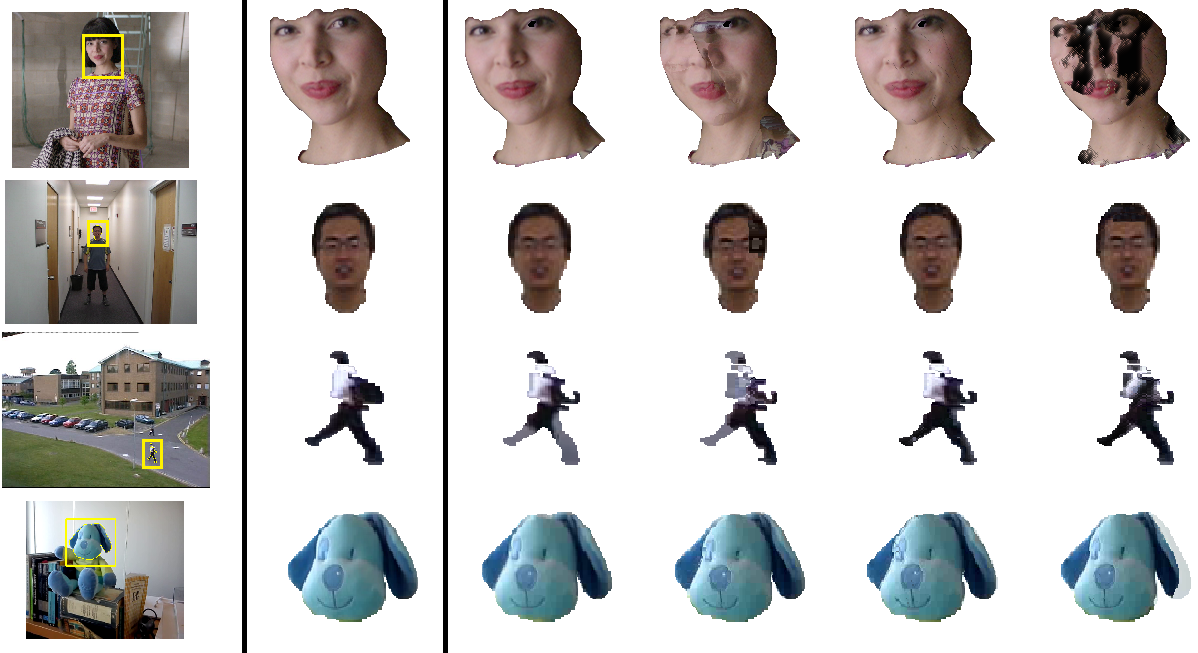
\includegraphics[width=1.0\textwidth]{../images/extrapolated.png}
      \caption{Extrapolation results from integrated flow in 4 sequences. In descending order: Amelia Retro, Boy, Walking, Puppy. From Left to Right: Annotated object, Backward object flow, Backward optical flow, Forward object flow, Backward optical flow.}
      \label{sample}
   \end{figure}
	\setlength{\belowcaptionskip}{-10pt}

To evaluate the performance of the object flow in comparison with optical flow techniques, we performed 
a number of experiments on several video sequences. We annotated an initial bounding box for the videos, 
and a segmentation contour of the interest object for every frame. The experiment measures the ability of the method to 
extrapolate an image from the initial frame and the integrated flow. For every pair of frames the video sequence, the PSNR between the annotated
current state of the object and the extrapolated images is computed. The Fig. \ref{sample} is a sample of the performed experiment, each column is an image generated from the given flow. 
Two types integration are evaluated, $From-the-reference$, or forward integration, and $To-the-reference$, or backward integration, as discused in \cite{c20}. So, for each row in the Fig. \ref{sample}, two columns correspond to the object flow, and two columns correspond to optical flow, with both types of integration.

The Fig. \ref{of_res} shows PSNR graphics for 4 different sequences. For every pair of frames an image is extrapolated, and the PSNR with the ground-truth object is computed.
The results are shown with both, Euler integration (Labelled as $forward$ in the figs.) of the used flow, 
and using the integration method described in \cite{c20}, labeled as $backward$ in the figures. The results show that the object flow methods are generally more precise than its optical flow 
counterparts. Moreover, the object flow method with backward integration usually performs much better than any other combination of techniques. For this experiment, the object flow is compared with the simple-flow optical-flow method. This experiment directly shows that the object flow concept is indeed capable of increasing accuracy of a given optical flow method. 

   \begin{figure}[hb]
      \centering
      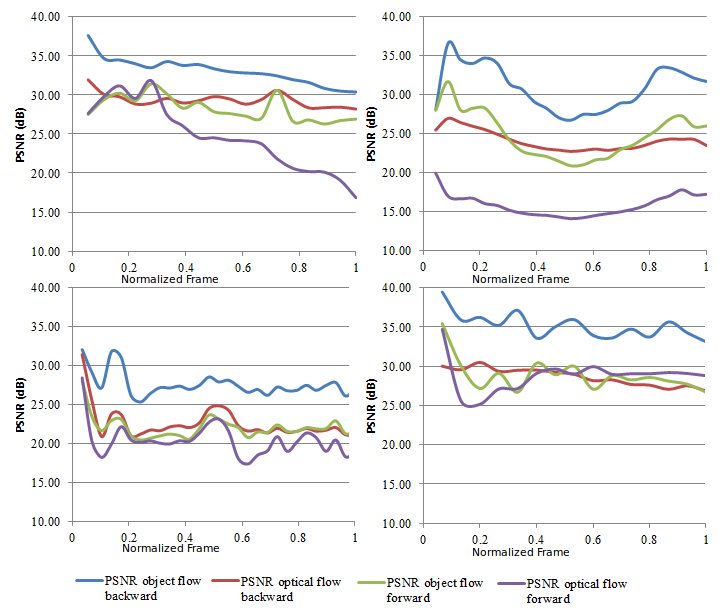
\includegraphics[width=0.925\textwidth]{../images/psnr_v2.png}
      \caption{PSNR graphs for extrapolated images using Object flow and the Simple Optical Flow for 4 sequences. From left to right and up to bottom: Puppy Seq.; Amelie Retro Seq.; Boy Seq.; Walking Seq.}
      \label{of_res}
   \end{figure}
	\setlength{\belowcaptionskip}{-10pt}


Now, in order to study how the object flow concept compares to several state of the art optical flow 
methods, another extrapolation experiment is performed. 
The Fig. \ref{compare2} presents a visual comparison between the object flow and several optical flow 
techniques in the Amelia sequence for object extrapolation, and the involved frames (the first and last used frames in the sequence). 
The Fig. \ref{of_res2} shows the PSNR results for every extrapolated frame in the full sequence, 
the object flow performs better than all the studied optical flow techniques.


   \begin{figure}[t]
      \centering
      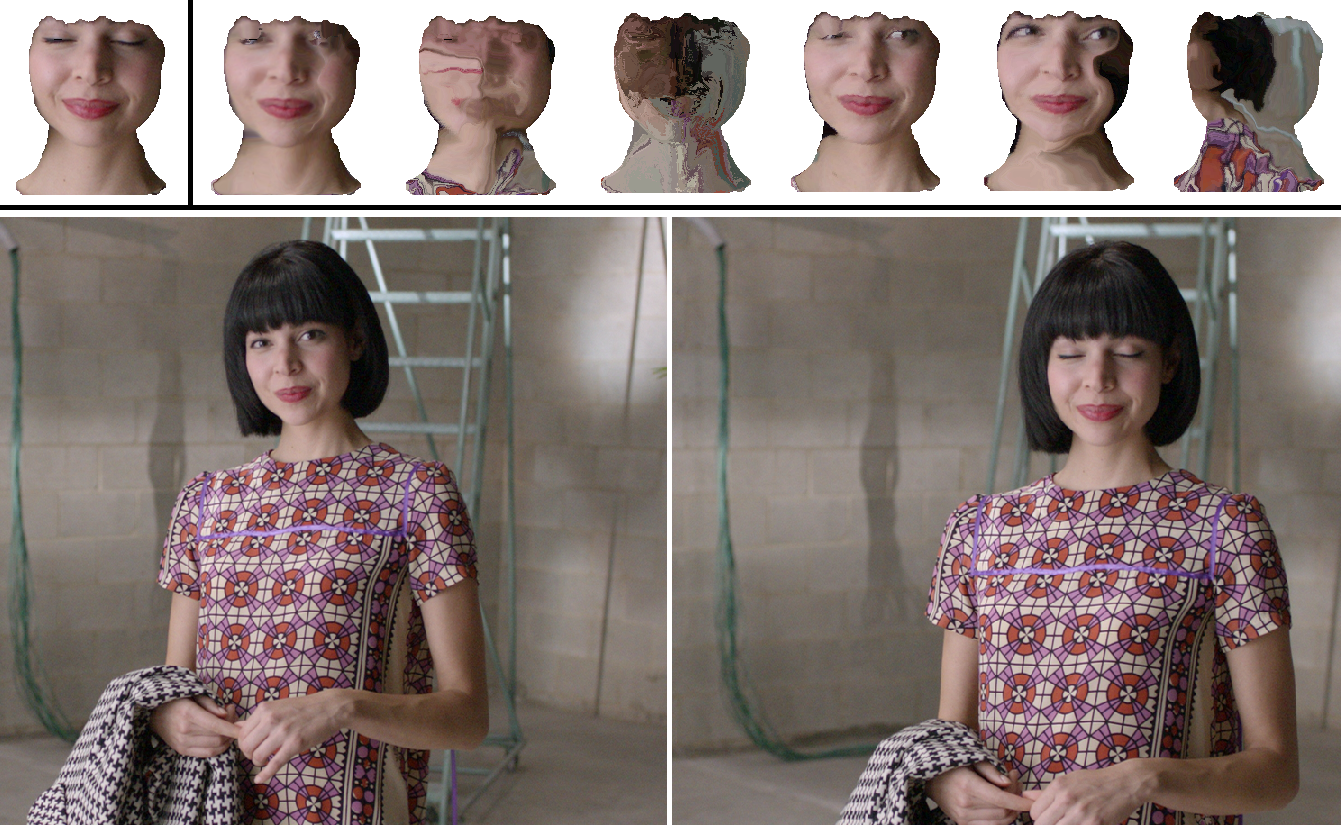
\includegraphics[width=0.925\textwidth]{../images/compare2.png}
      \caption{Top: The first frame and the accumulated flows are used to extrapolate objects in the frame number 30. The used methods from left to right: Groundtruth object, Object flow, TVL1, Block Matching, Brox, Farneback and Simple Flow. 
		Bottom: First and frame\#30. The extrapolations are performed using backward accumulation of the flows.}
      \label{compare2}
   \end{figure}
	\setlength{\belowcaptionskip}{-10pt}


Observe that the object details are lost in comparison with the ground-truth object image (Fig. \ref{compare2}). For example, the closed eyes detail is missing in the most of the optical 
flow methods. Furthermore, several of the methods lost any significance, and the output barely holds any resemblance with the original image. This is possibly the result of a couple of details that are naturally better attacked with the object flow: 
long motion (the tracker always centers the object in any given frame), and smoothness prior (the segmentation mask is a 
good delimitation to establish this prior).

   \begin{figure}[th]
      \centering
      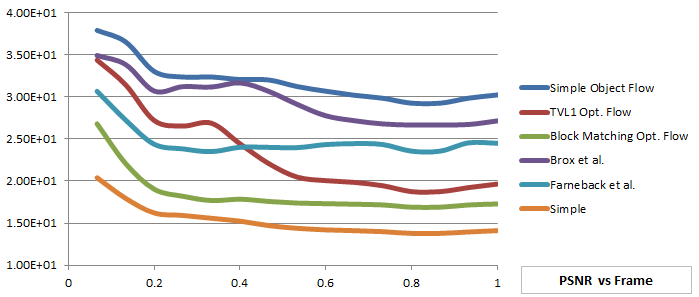
\includegraphics[width=1.0\textwidth]{../images/psnr2.png}
      \caption{PSNR graphs for extrapolated images using Object flow and the different Optical Flow techniques for the Amelia sequence. }
      \label{of_res2}
   \end{figure}
	\setlength{\belowcaptionskip}{-10pt}

\section{Implementation details}

A framework to combine state-of-the-art optical flow and tracking methods was implemented in C++, and using the OpenCV 3.0 and Eigen 3 libraries. 
The framework consists on 3 main virtual classes: Tracker, 
OpticalFlow and ObjectFlow. The function of these base classes is to define the interfaces for several implementations of each algorithm. For instance, 
the implemented or adopted tracking methods are:

\begin{itemize}
  \item Color Histograms Mean-Shift,
  \item Color Spatiograms Mean-Shift,
  \item Color Spatiograms Based Particle Filter,
  \item Color Histogram Cam-Shift,
  \item Multiple Instance Learning Tracker,
  \item Boosting Tracker,
  \item Struck Tracker,
  \item TLD Tracker.
\end{itemize}

And the used optical flow methods are:

\begin{itemize}
  \item Lucas-Kanade,
  \item Horn,
  \item TV-L1,
  \item Fast Block Matching, 
  \item Simple Flow,
  \item Farneback,
  \item Affine Transformation based on Keypoint matching,
  \item Thin Plate Spline Transformation based on Keypoint matching,
  \item Brox method.
\end{itemize}

The Fig. \ref{class} shows a simplified class diagram for the implemented framework. It can be appreciated that all major interfaces inherit from the {\it cv::Algorithm} class to provide 
implementation flexibilities through instantation by smart pointers ({\it cv::Ptr}) and to mantain organization in the interfaces. 

   \begin{figure}[thbp]
      \centering
      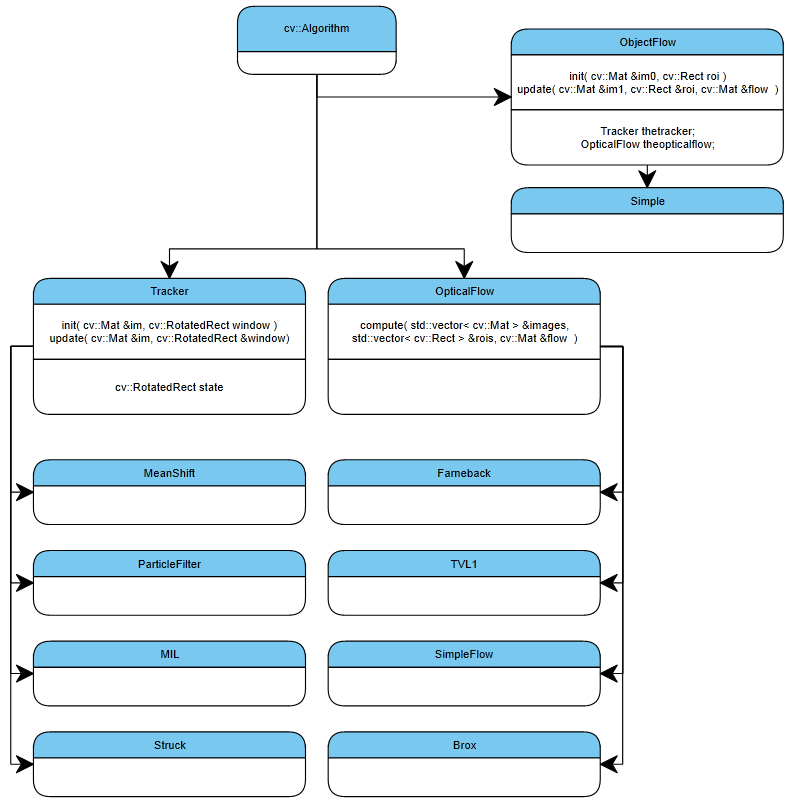
\includegraphics[width=0.925\textwidth]{../images/ClassDiagram.png}
      \caption{Simplified class diagram for the implemented workflow.}
      \label{class}
   \end{figure}
	\setlength{\belowcaptionskip}{-10pt}

